\section{moeo\-Easy\-EA$<$ MOEOT $>$::eo\-Dummy\-Select Class Reference}
\label{classmoeoEasyEA_1_1eoDummySelect}\index{moeoEasyEA::eoDummySelect@{moeoEasyEA::eoDummySelect}}
a dummy select  


{\tt \#include $<$moeo\-Easy\-EA.h$>$}

Inheritance diagram for moeo\-Easy\-EA$<$ MOEOT $>$::eo\-Dummy\-Select::\begin{figure}[H]
\begin{center}
\leavevmode
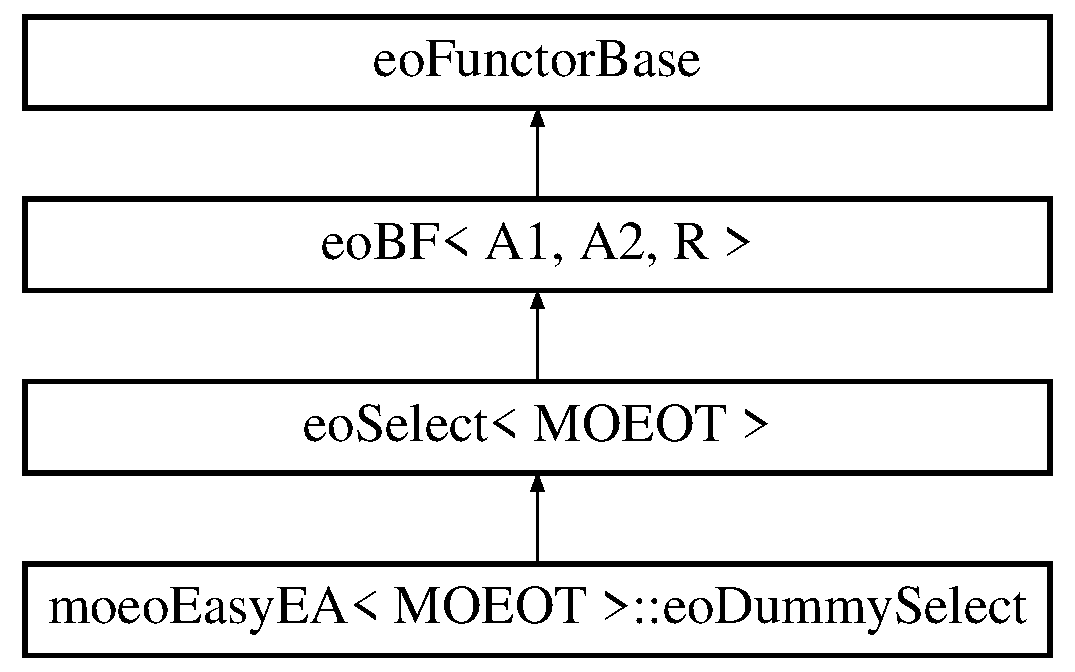
\includegraphics[height=4cm]{classmoeoEasyEA_1_1eoDummySelect}
\end{center}
\end{figure}
\subsection*{Public Member Functions}
\begin{CompactItemize}
\item 
void \bf{operator()} (const \bf{eo\-Pop}$<$ MOEOT $>$ \&, \bf{eo\-Pop}$<$ MOEOT $>$ \&)\label{classmoeoEasyEA_1_1eoDummySelect_32207d2ed997aa90ba9f32f5625b63d6}

\begin{CompactList}\small\item\em the dummy functor \item\end{CompactList}\end{CompactItemize}


\subsection{Detailed Description}
\subsubsection*{template$<$class MOEOT$>$ class moeo\-Easy\-EA$<$ MOEOT $>$::eo\-Dummy\-Select}

a dummy select 



Definition at line 204 of file moeo\-Easy\-EA.h.

The documentation for this class was generated from the following file:\begin{CompactItemize}
\item 
moeo\-Easy\-EA.h\end{CompactItemize}
